\section{Object Selection Criteria}
\label{sec:criteria}
We create color-color criteria to generate a catalog of AGB candidates. We seek to maximize AGB completeness while minimizing contamination from non-AGB objects to beneath the 1\% level.

The color-color criteria for AGB selection are as follows:
\begin{align} 
(J-K_s) > 1.1\label{eq:criteria1}\\
(W2-W3) > 0.3\label{eq:criteria2}\\
(W3-W4) < -0.83(W2-W3) + 3.37\label{eq:criteria3}
\end{align}
The criteria in (\ref{eq:criteria1}) and (\ref{eq:criteria2}) are primarily concerned with rejecting objects from the stellar locus, and other stars whose NIR spectra are dominated by the Rayleigh-Jeans tail (many covered by the sample of galaxies). (\ref{eq:criteria3}) also rejects stars from the stellar locus, but primarily functions to remove IR-bright extragalactic sources.

\noindent Sample completeness $\eta$ is defined as
\begin{eqnarray*}
\eta &=& \frac{N - n_\text{missed}}{N}
\end{eqnarray*}
where $N$ is the total number of objects in the sample, and $n_\text{missed}$ is the number of objects outside of the applied boundaries. Figure~\ref{fig:completeness} shows the distribution of sample completeness amongst AGB sources after the application of the above criteria. The vast majority (79.07\%) of Galactic AGB stars is recovered after criteria (\ref{eq:criteria1}), (\ref{eq:criteria2}), and (\ref{eq:criteria3}) are applied. The largest losses occur at the edges of the Galactic disk ($\lvert b\rvert\approx10^\circ$) and in regions of high stellar number density both in the Galaxy and the Magellanic Clouds. In the color-color diagrams, selection completeness degrades near the borders of the selction area, as objects that straddle these boundaries may exhibit enough emission in other color-color spaces to be removed by our criteria. Of the remaining sample of 5,709 objects, 52.94\% lie within the disk ($\lvert b\rvert<10^\circ$).

\begin{figure}[h]
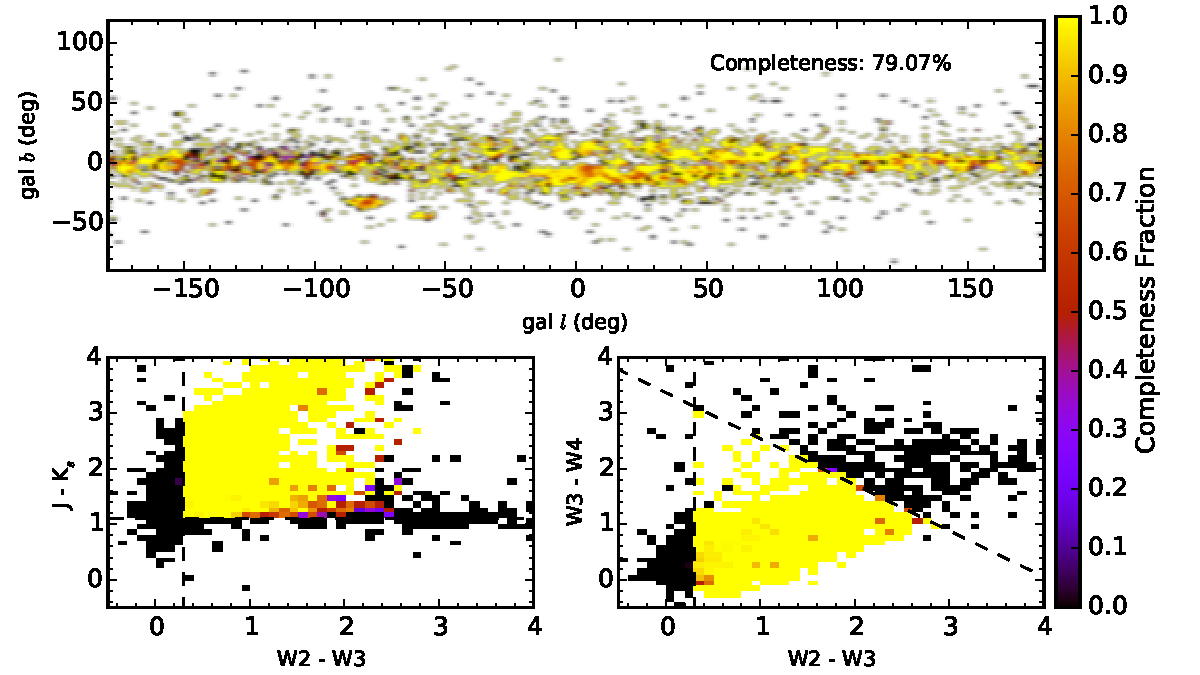
\includegraphics[width=6.7in]{figs/completeness_map.pdf}
\caption{Sample selection completeness maps in ($l,b$) space (\emph{top}) and the color-color space of our selection criteria (\emph{bottom}). Color scale shows the completeness fraction per bin, with 4-deg$^2$ bins on the Galactic map and 0.1 dex bins on each axis of the color-color diagrams. Selection criteria are shown as dashed lines.\label{fig:completeness}}
\end{figure}

\cite{2013sdmm.book.....I} defines sample contamination as
\begin{eqnarray*}
\epsilon &=& \frac{n_\text{spurious}}{n_\text{selected}}.
\end{eqnarray*}
where $n_\text{spurious}$ is the number of spurious sources and $n_\text{selected} = N + n_\text{spurious}$. The contamination map is shown in Figure~\ref{fig:contamination}. Most bins in Figure~\ref{fig:contamination} exhibit 0\% contamination, with the overall contamination level at 0.38\%. What contaminants do remain exist primarily at the very fringes of the AGB star distribution in ($J-K_S$) vs ($W2 - W3$) space and near the redder boundary in ($W3-W4$) vs ($W2 - W3$), where bluer extragalactic sources creep into the selection region. The results of the applied critiera on both the collective AGB and contaminant samples are summarized in Table~\ref{tab:completeness}.

\begin{figure}[h]
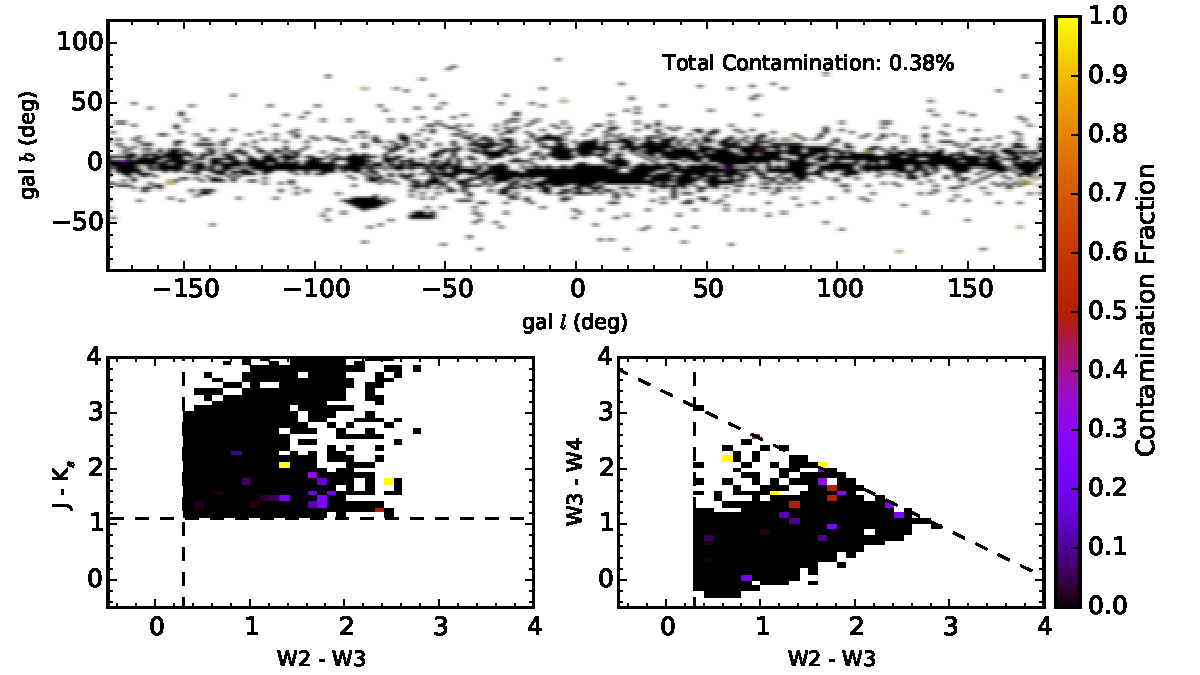
\includegraphics[width=6.7in]{figs/contamination_map.pdf}
\caption{Sample contamination in Galactic ($l,b$) space (\emph{top}) and color-color space (\emph{bottom}). Boundaries and binning the same as Fig~\ref{fig:completeness}.\label{fig:contamination}}
\end{figure}

%One large issue with the boundaries are the O-rich AGB stars.  Either the objects from the OGLE O-rich AGB star catalog were mostly mis-matched to WISE, taking on colors of the stellar locus, or the issue is more physical.  It could be that the warm O-rich AGB photospheres are still visible and not heavily enshrouded in dust, thus appearing similar to Main Sequence stars in the NIR. Previous work on warm O-rich AGB stars has shown that their circumstellar shells are not prominent, and their NIR photometry reflects the Rayleigh Jeans tail of a cool 2000-4000K blackbody \citep{1974ApJ...189...89D}. 

\begin{table}[h]
    \begin{center}
        \caption{Sample Selection Completeness and Contamination}
        \scalebox{0.85}{
            \begin{tabular}{l c c c c c c}
		\hline
		Population & SIMBAD AGB* & C* & Mira & OH/IR & S* \\ 
		Completeness & 89.62\% & 72.11\% & 95.62\% & 39.53\% & 22.31\% \\ 
		\hline
		Population & MACHO seq1 & seq2 & seq3 & seq4 \\ 
		Completeness & 88.45\% & 81.08\% & 28.77\% & 14.75\% \\ 
		\hline
		Population & OGLE-III C-rich & O-rich & \textbf{All AGB Stars} \\ 
		Completeness & 73.09\% & 70.68\% & \textbf{79.07\%} \\ 
		\hline
		Population & DR12 SSPP & DR7 LRG & Galaxies & QSO & AGN \\ 
		Contamination & 0.56\% & 0.00\% & 0.00\% & 0.07\% & 	0.00\% \\ 
		\hline

                \label{tab:completeness}
            \end{tabular}}    
    \end{center}
\end{table}


